% Provenance (never printed): cycle 3 / 6e "La planete Terre" (rocks and
% minerals; the three rock families; recognising common rocks); see
% sources/book1/PROVENANCE.md. Book 1, grade 6, chapter 3.
% Vocabulary guard: "magma" not before g7.2 (here "molten rock");
% "sediment" not before g7.4 (here "grains of sand and mud").
\chapter{Batuan dan Mineral}\label{ch:g6:rocks-and-minerals}

Sam membungkuk di atas meja dapur sambil memegang kaca pembesar. Batu yang
mengilap itu, yang dari jauh tampak kelabu, berubah menjadi kerumunan
bintik: ada yang merah muda, ada yang putih, ada yang kelabu seperti kaca,
dan ada yang hitam kecil-kecil yang berkilau ketika terkena cahaya. Setiap
bintik mempunyai sisi-sisi yang datar dan mengilap, dan bintik-bintik itu
saling mengunci seperti kepingan puzzle. Apakah bintik-bintik itu?

\begin{omfigure}
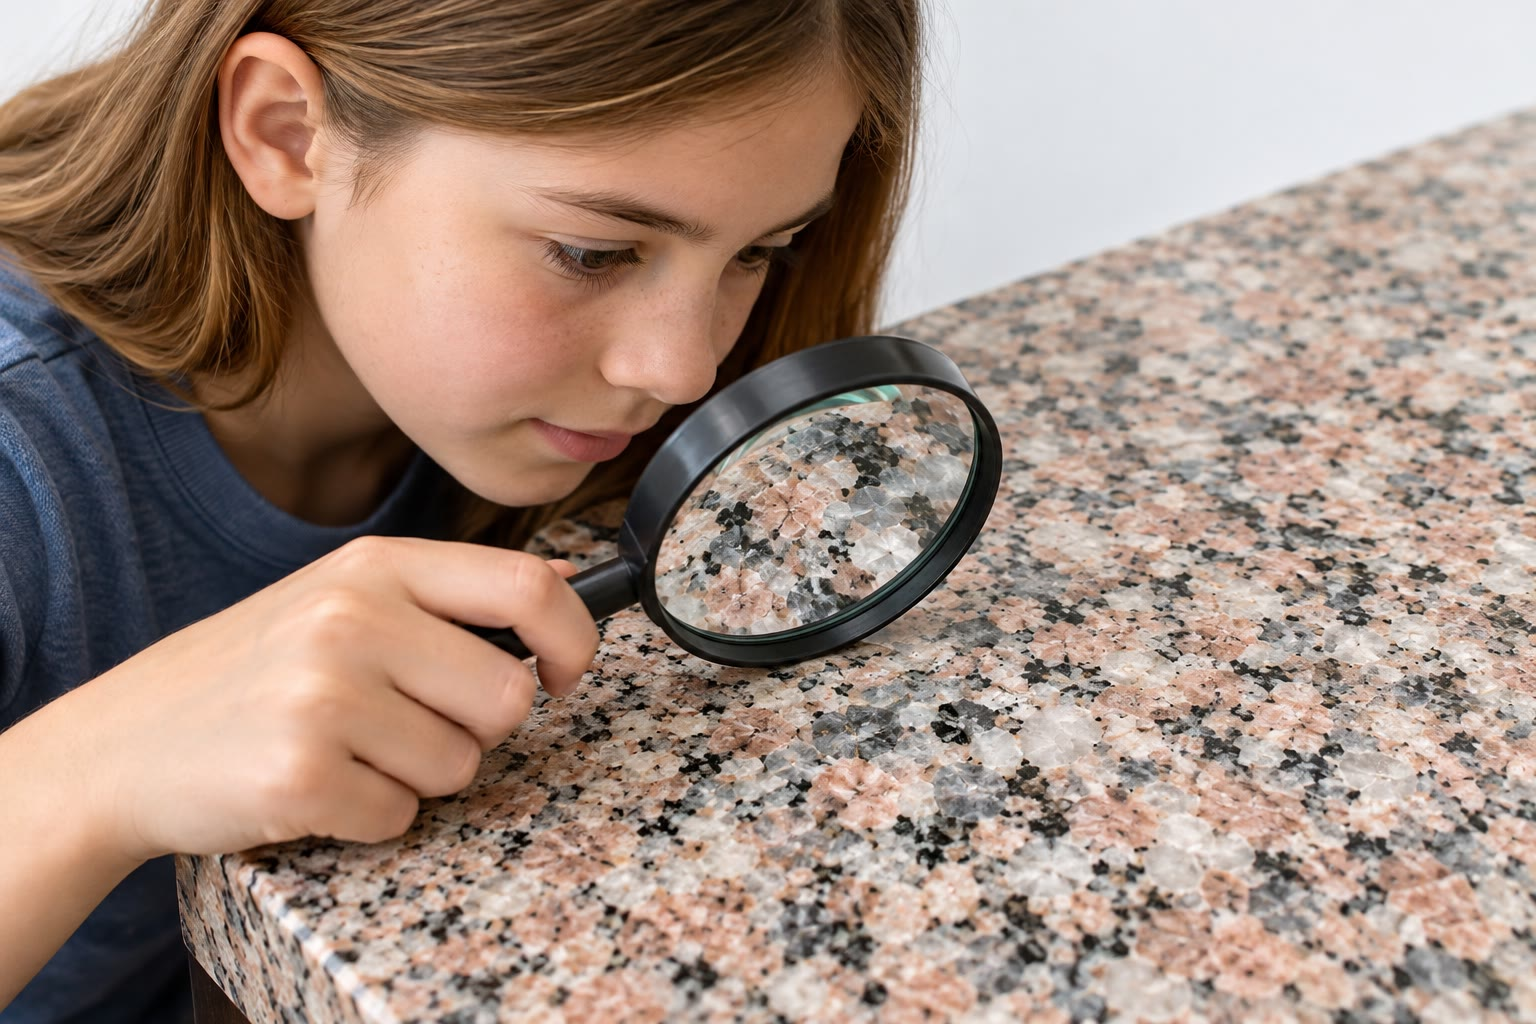
\includegraphics[width=0.6\linewidth]{images/book1/ai/g6-hand-lens-worktop.jpg}

{\small Mengamati meja dapur dari batu berbintik dengan kaca pembesar.
(Ilustrasi AI.)}
\end{omfigure}

\begin{recall}
\omterm{def:g3:stones-pebbles-sand:rock}{Batuan} adalah bahan keras penyusun kerak Bumi: \omterm{def:g3:stones-pebbles-sand:rock}{batuan} dapat pecah menjadi
batu, digulingkan oleh \omterm{def:g1:landscapes-around-us:water}{sungai} menjadi \omterm{def:g3:stones-pebbles-sand:pebble}{kerakal}, dan digerus menjadi \omterm{def:g3:stones-pebbles-sand:sand}{pasir}
(\cref{ch:g3:stones-pebbles-sand}). Air, es, dan angin mengikis \omterm{def:g3:stones-pebbles-sand:rock}{batuan}
(\omterm{def:g5:water-shapes-the-land:weathering}{pelapukan}), mengangkut kepingannya (\omterm{def:g5:water-shapes-the-land:erosion}{erosi}), dan menjatuhkannya lebih jauh
di bawah (\omterm{def:g5:water-shapes-the-land:deposition}{pengendapan}) (\cref{ch:g5:water-shapes-the-land}). Di \omterm{def:g4:volcanoes-earthquakes-first-look:volcano}{gunung api},
\omterm{def:g3:stones-pebbles-sand:rock}{batuan} yang meleleh keluar sebagai \omterm{def:g4:volcanoes-earthquakes-first-look:eruption}{lava}
(\cref{ch:g4:volcanoes-earthquakes-first-look}).
\end{recall}

\section{Batuan tersusun dari mineral}

Bintik-bintik pada meja dapur itu adalah \omterm{def:g6:rocks-and-minerals:mineral}{mineral}, dan batunya adalah granit.

\begin{definition}[Mineral]\label{def:g6:rocks-and-minerals:mineral}
Yang disebut \emph{mineral}\index{mineral} adalah zat padat alami, yang tidak
dibuat oleh makhluk hidup, yang susunannya selalu sama dan atom-atomnya
tersusun secara teratur. Sebuah \emph{\omterm{def:g3:stones-pebbles-sand:rock}{batuan}} tersusun dari satu mineral
atau, lebih sering, dari beberapa mineral yang melekat menjadi satu.
% ledger: usgs:mineral-rock
\end{definition}

Granit sebagian besar tersusun dari tiga \omterm{def:g6:rocks-and-minerals:mineral}{mineral}: \emph{feldspar} (merah
muda atau putih), \emph{kuarsa} (kelabu dan seperti kaca), dan \emph{mika}
(hitam atau keperakan, berupa serpihan tipis yang mengilap). \omterm{def:g3:stones-pebbles-sand:rock}{Batuan} lain
tersusun dari satu \omterm{def:g6:rocks-and-minerals:mineral}{mineral} saja: batu kapur, misalnya, hampir seluruhnya
tersusun dari kalsit.
% ledger: nps:granite-minerals, usgs:mineral-rock

\begin{omfigure}
\begin{minipage}[c]{0.5\linewidth}\centering
\begin{tikzpicture}
  \begin{axis}[axis equal image, hide axis, width=\linewidth,
      xmin=0, xmax=6, ymin=0, ymax=4]
    \addplot[fill=orange!35!pink, draw=black!55, line width=0.4pt]
      table {figdata/out/grade-6-granite_mosaic-feldspar.dat};
    \addplot[fill=black!12, draw=black!55, line width=0.4pt]
      table {figdata/out/grade-6-granite_mosaic-quartz.dat};
    \addplot[fill=black!85, draw=black!55, line width=0.4pt]
      table {figdata/out/grade-6-granite_mosaic-mica.dat};
  \end{axis}
\end{tikzpicture}

{\small \tikz\fill[orange!35!pink, draw=black!55] (0,0) rectangle (0.25,0.18); feldspar\quad
\tikz\fill[black!12, draw=black!55] (0,0) rectangle (0.25,0.18); kuarsa\quad
\tikz\fill[black!85] (0,0) rectangle (0.25,0.18); mika}
\end{minipage}\hfill
\begin{minipage}[c]{0.46\linewidth}\centering
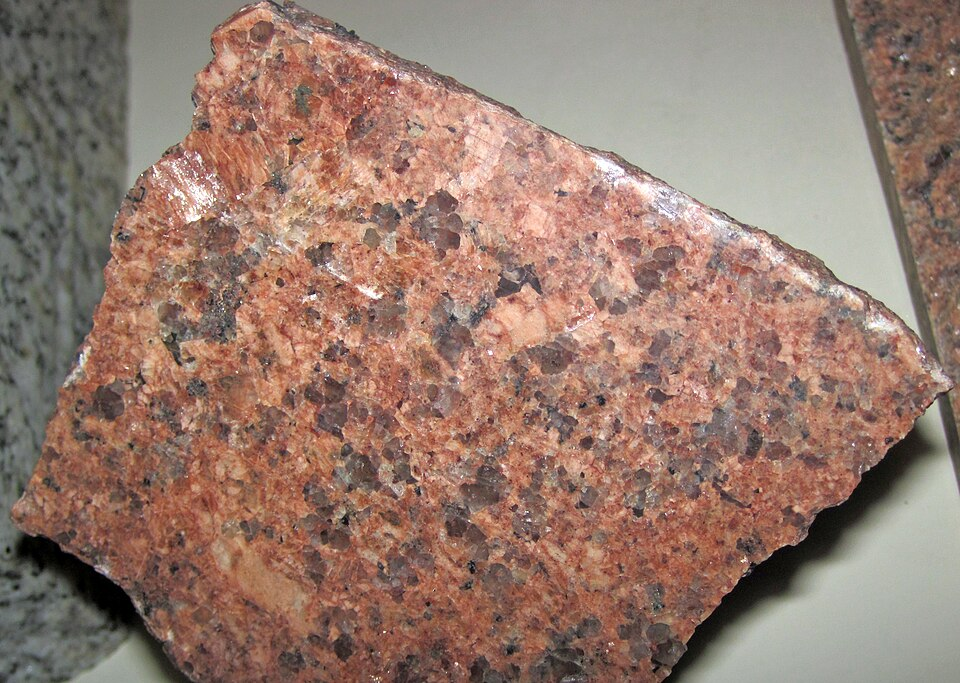
\includegraphics[width=\linewidth]{images/book1/g6-granite.jpg}
\end{minipage}

\smallskip
{\small Kiri: granit digambar sebagai mozaik butiran, setiap butir satu
\omterm{def:g6:rocks-and-minerals:mineral}{mineral} (perbesaran, tidak menurut skala). Kanan: granit merah muda yang
sebenarnya, kira-kira seukuran tangan. (Foto: James St.~John, CC BY 2.0,
melalui Wikimedia Commons.)}
% ledger: nps:granite-minerals, commons:jsj-rocks (figdata/grade-6/granite_mosaic.py)
\end{omfigure}

\section{Kristal}

Di bawah kaca pembesar, banyak butir \omterm{def:g6:rocks-and-minerals:mineral}{mineral} memperlihatkan sisi-sisi yang
datar dan mengilap serta rusuk-rusuk yang lurus. Di tempat sebuah \omterm{def:g6:rocks-and-minerals:mineral}{mineral}
mempunyai ruang untuk tumbuh dengan bebas, di dalam rongga \omterm{def:g3:stones-pebbles-sand:rock}{batuan}, \omterm{def:g6:rocks-and-minerals:mineral}{mineral}
itu membentuk kristal: zat padat berbentuk teratur yang dibatasi oleh
bidang-bidang datar. Bentuknya berasal dari susunan atom-atomnya yang
teratur, yang dipelajari dalam buku kimia. Kristal kuarsa, misalnya,
berupa tiang bersisi enam yang ujungnya runcing; kristal mika terbelah
menjadi lembaran yang lebih tipis daripada kertas.

\begin{omfigure}
\begin{minipage}[c]{0.2\linewidth}\centering
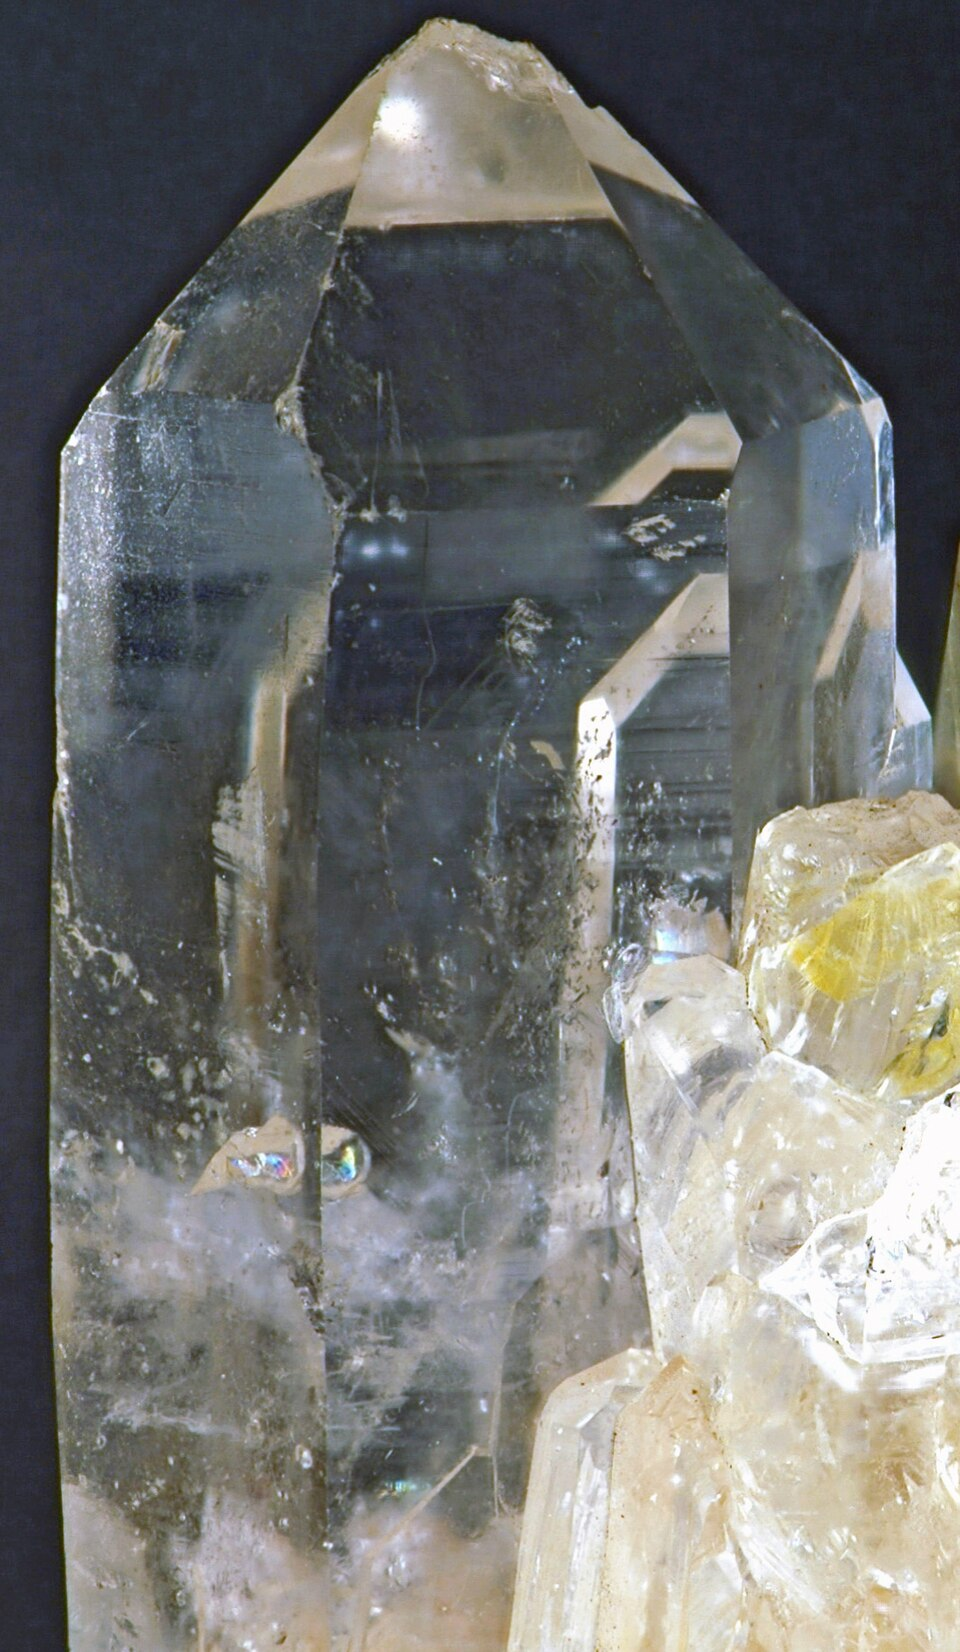
\includegraphics[height=4.2cm]{images/book1/g6-quartz.jpg}
\end{minipage}\hfill
\begin{minipage}[c]{0.44\linewidth}\centering
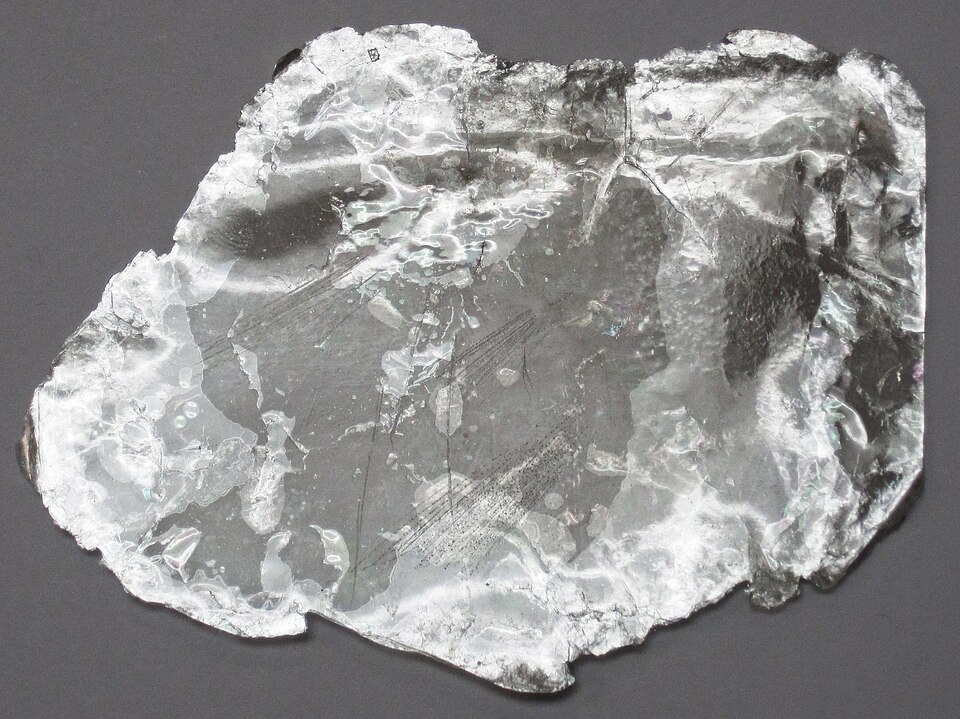
\includegraphics[height=4.2cm]{images/book1/g6-mica.jpg}
\end{minipage}\hfill
\begin{minipage}[c]{0.28\linewidth}
{\small Kiri: sebuah kristal kuarsa, dengan bidang-bidangnya yang datar.
Kanan: selembar mika, \omterm{def:g6:rocks-and-minerals:mineral}{mineral} yang terbelah menjadi serpihan yang sangat
tipis. (Foto: James St.~John, CC BY 2.0, melalui Wikimedia Commons.)}
% ledger: commons:jsj-rocks
\end{minipage}
\end{omfigure}

Di dalam granit, butiran-butirannya tumbuh sambil saling berdesakan, jadi
bentuknya tidak rapi: butiran itu saling mengunci seperti puzzle. Ukurannya
menceritakan sebuah kisah. Granit terbentuk jauh di bawah tanah, tempat
\omterm{def:g3:stones-pebbles-sand:rock}{batuan} yang meleleh mendingin dengan sangat lambat: butiran-butirannya
mempunyai waktu untuk tumbuh cukup besar sehingga dapat dilihat dengan mata.
\omterm{def:g3:stones-pebbles-sand:rock}{Batuan} yang meleleh dan mendingin dengan cepat di permukaan, sebagai \omterm{def:g4:volcanoes-earthquakes-first-look:eruption}{lava},
menghasilkan \omterm{def:g3:stones-pebbles-sand:rock}{batuan} dengan butiran yang terlalu kecil untuk dilihat.
% ledger: usgs:mineral-rock

\section{Tiga keluarga batuan}

Para ahli geologi mengelompokkan \omterm{def:g3:stones-pebbles-sand:rock}{batuan} menjadi tiga keluarga, bukan menurut
warnanya, melainkan menurut cara terbentuknya.

\begin{definition}[Tiga keluarga batuan]\label{def:g6:rocks-and-minerals:rock-families}
Yang disebut \emph{batuan beku}\index{batuan beku} terbentuk ketika \omterm{def:g3:stones-pebbles-sand:rock}{batuan}
yang meleleh mendingin dan menjadi padat: granit jauh di bawah tanah, basal
dari \omterm{def:g4:volcanoes-earthquakes-first-look:eruption}{lava}. Yang disebut \emph{batuan sedimen}\index{batuan sedimen}
terbentuk di permukaan Bumi dari butiran \omterm{def:g3:stones-pebbles-sand:sand}{pasir} dan \omterm{def:g3:stones-pebbles-sand:sand}{lumpur}, atau dari
cangkang makhluk hidup, yang diendapkan berlapis-lapis lalu mengeras: batu
pasir, serpih, batu kapur. Yang disebut
\emph{batuan metamorf}\index{batuan metamorf} adalah \omterm{def:g3:stones-pebbles-sand:rock}{batuan} yang telah
berubah bentuk, tanpa meleleh, oleh panas dan tekanan jauh di bawah tanah:
marmer (dari batu kapur), batu sabak (dari serpih).
% ledger: usgs:mineral-rock, usgs:sedimentary, usgs:metamorphic, geo:marble, geo:slate
\end{definition}

Kata \emph{beku} dalam namanya berarti bahwa \omterm{def:g3:stones-pebbles-sand:rock}{batuan} ini terbentuk ketika
\omterm{def:g3:stones-pebbles-sand:rock}{batuan} yang meleleh membeku menjadi padat; dalam banyak bahasa lain, namanya
berasal dari kata Latin untuk api. \omterm{def:g6:rocks-and-minerals:rock-families}{Batuan sedimen} sering memperlihatkan lapisan-lapisan,
yang satu di atas yang lain, seperti halaman-halaman buku. \omterm{def:g6:rocks-and-minerals:rock-families}{Batuan metamorf}
sering kali tertekan dan terlipat; sebagian, seperti batu sabak, terbelah
menjadi lembaran-lembaran yang datar.
% ledger: usgs:mineral-rock, usgs:sedimentary, usgs:metamorphic

Banyak \omterm{def:g6:rocks-and-minerals:rock-families}{batuan sedimen} tersusun dari butiran yang kamu kelompokkan menurut
ukurannya dalam \cref{ch:g3:stones-pebbles-sand}: \omterm{def:g3:stones-pebbles-sand:pebble}{kerakal} dan \omterm{def:g3:stones-pebbles-sand:pebble}{kerikil},
\omterm{def:g3:stones-pebbles-sand:sand}{pasir}, \omterm{def:g3:stones-pebbles-sand:sand}{lumpur}. Setelah terkubur, butiran-butiran itu kehilangan airnya dan
direkatkan oleh semen alami. Ukuran butirannya memberi nama \omterm{def:g3:stones-pebbles-sand:rock}{batuan} itu.
% ledger: usgs:sedimentary, usgs:wentworth

\begin{omfigure}
\begin{tikzpicture}[
    col/.style={draw=black!60, rounded corners=2pt, minimum width=3.6cm, minimum height=1.9cm},
    lab/.style={font=\scriptsize, align=center}]
  % gravel -> conglomerate
  \node[col, fill=omLithCongl!50] (g) at (0,0) {};
  \foreach \x/\y/\r in {-1.2/0.4/0.32, -0.4/-0.3/0.4, 0.5/0.35/0.3, 1.25/-0.35/0.33, 0.2/-0.55/0.18, -1.3/-0.5/0.22}
    \fill[gray!55, draw=black!60] (\x,\y) circle (\r);
  \node[lab, above=2pt] at (g.north) {\textbf{kerikil}\\ lebih dari 2~mm};
  \node[lab, below=3pt] (cg) at (g.south) {$\downarrow$ terkubur dan tersemen\\ \textbf{konglomerat}};
    % sand -> sandstone
  \pgfmathsetseed{7}

  \node[col, fill=omLithSand!60] (s) at (4.2,0) {};
  \foreach \i in {1,...,70} \fill[brown!60!black] ({4.2+1.65*rand},{0.82*rand}) circle (0.045);
  \node[lab, above=2pt] at (s.north) {\textbf{pasir}\\ 2~mm sampai $\frac{1}{16}$~mm};
  \node[lab, below=3pt] at (s.south) {$\downarrow$ terkubur dan tersemen\\ \textbf{batu pasir}};
  % mud -> shale
  \node[col, fill=omLithShale!70] (m) at (8.4,0) {};
  \foreach \y in {-0.75,-0.5,...,0.8} \draw[black!35, line width=0.3pt] (6.75,\y) -- (10.05,\y);
  \node[lab, above=2pt] at (m.north) {\textbf{lumpur} (lanau dan lempung)\\ kurang dari $\frac{1}{16}$~mm};
  \node[lab, below=3pt] at (m.south) {$\downarrow$ terkubur dan tertekan\\ \textbf{serpih}};
\end{tikzpicture}

{\small Tiga \omterm{def:g6:rocks-and-minerals:rock-families}{batuan sedimen} yang dinamai menurut ukuran butirannya
(butiran sangat diperbesar; \omterm{def:g3:stones-pebbles-sand:sand}{pasir} digambar pada skala kotak, \omterm{def:g3:stones-pebbles-sand:pebble}{kerikil} lebih
besar).}
% ledger: usgs:wentworth, usgs:sedimentary
\end{omfigure}

\begin{inthefield}[Membaca batu-batu sebuah kota]
Kota-kota adalah koleksi \omterm{def:g3:stones-pebbles-sand:rock}{batuan} di udara terbuka. Berjalanlah bersama orang
dewasa melewati tembok tua, anak tangga, patung, muka gereja, dan
ubin jalan, lalu amatilah dengan teliti, tanpa menggores atau memecahkan
apa pun. Sebagian tepi trotoar dan anak tangga terbuat dari granit:
carilah kuarsanya yang seperti kaca dan mikanya yang mengilap. Banyak tembok
tua dan muka bangunan terbuat dari batu kapur atau batu pasir: carilah
cangkang, atau gosoklah remah batu pasir yang jatuh dengan ujung jarimu
untuk merasakan \omterm{def:g3:stones-pebbles-sand:sand}{pasirnya}. Atap mungkin terbuat dari batu sabak, yang
terbelah menjadi lembaran tipis. Catatlah di buku catatan tempat setiap
batu, warnanya, butirannya, dan keluarga \omterm{def:g3:stones-pebbles-sand:rock}{batuan} yang menurutmu tepat; foto
membantu untuk membandingkannya nanti dengan tabel dalam bab ini.
\end{inthefield}

\section{Siklus batuan}

\omterm{def:g3:stones-pebbles-sand:rock}{Batuan} tidak abadi. \omterm{def:g1:landscapes-around-us:landform}{Gunung} granit perlahan-lahan melapuk; butiran-butirannya
diangkut oleh \omterm{def:g1:landscapes-around-us:water}{sungai} ke \omterm{def:g2:water-on-earth:ocean}{laut} dan diendapkan di sana berlapis-lapis; makin
lama makin dalam terkubur, lapisan-lapisan itu mengeras menjadi batu pasir.
Jika batu pasir itu terbawa lebih dalam lagi, panas dan tekanan mengubahnya
menjadi \omterm{def:g6:rocks-and-minerals:rock-families}{batuan metamorf}; lebih dalam lagi, \omterm{def:g3:stones-pebbles-sand:rock}{batuan} itu dapat meleleh, dan
\omterm{def:g3:stones-pebbles-sand:rock}{batuan} yang meleleh itu, ketika mendingin, membentuk \omterm{def:g6:rocks-and-minerals:rock-families}{batuan beku} yang baru.
Sedikit demi sedikit, selama jutaan tahun, bahan penyusun \omterm{def:g3:stones-pebbles-sand:rock}{batuan} terus
berputar.
% ledger: usgs:sedimentary, usgs:metamorphic

\begin{definition}[Siklus batuan]\label{def:g6:rocks-and-minerals:rock-cycle}
Yang disebut \emph{siklus batuan}\index{siklus batuan} adalah perjalanan tanpa
akhir yang membuat \omterm{def:g3:stones-pebbles-sand:rock}{batuan} dari setiap keluarga perlahan-lahan berubah
menjadi \omterm{def:g3:stones-pebbles-sand:rock}{batuan} dari keluarga lain: oleh \omterm{def:g5:water-shapes-the-land:weathering}{pelapukan} dan \omterm{def:g5:water-shapes-the-land:erosion}{erosi} di permukaan,
oleh penguburan dan pengerasan, oleh panas dan tekanan, oleh pelelehan dan
pendinginan.
\end{definition}

\begin{omfigure}
\begin{tikzpicture}[
    fam/.style={draw, rounded corners=4pt, thick, align=center, minimum width=3.2cm,
                minimum height=1.0cm, font=\small\bfseries},
    stage/.style={draw, dashed, rounded corners=4pt, align=center, minimum width=3.0cm,
                  minimum height=0.9cm, font=\small},
    arr/.style={-{Stealth[length=2.6mm]}, thick},
    lab/.style={font=\scriptsize, align=center, fill=white, inner sep=1.5pt}]
  \node[fam, fill=omLithGranite!60] (ign) at (0,3.6) {batuan beku\\[-1pt]{\normalfont\scriptsize granit, basal}};
  \node[stage, fill=orange!15] (grains) at (6.6,3.6) {butiran pasir\\dan lumpur};
  \node[fam, fill=omLithSand!70] (sed) at (6.6,0) {batuan sedimen\\[-1pt]{\normalfont\scriptsize batu pasir, serpih, batu kapur}};
  \node[fam, fill=omLithSchist!60] (met) at (0,0) {batuan metamorf\\[-1pt]{\normalfont\scriptsize marmer, batu sabak}};
  \node[stage, fill=red!12] (melt) at (-4.2,1.8) {batuan yang meleleh\\jauh di dalam};
  \draw[arr] (ign) -- node[lab, above] {pelapukan\\dan erosi} (grains);
  \draw[arr] (grains) -- node[lab, right] {diendapkan berlapis,\\terkubur, mengeras} (sed);
  \draw[arr] (sed) -- node[lab, below=2pt] {panas dan tekanan,\\jauh di dalam} (met);
  \draw[arr] (met) -- node[lab, below left] {pelelehan} (melt);
  \draw[arr] (melt) -- node[lab, above left] {pendinginan} (ign);
  \draw[arr, black!55] (met.north east) to[bend left=12] node[lab, pos=0.45, left=4pt, text=black!60] {pelapukan} ([xshift=-6pt]grains.south west);
  \draw[arr, black!55] (sed.north west) to[bend left=10] (grains.south west);
\end{tikzpicture}

{\small \omterm{def:g6:rocks-and-minerals:rock-cycle}{Siklus batuan}. Setiap panah memerlukan waktu ribuan sampai jutaan
tahun. \omterm{def:g3:stones-pebbles-sand:rock}{Batuan} apa pun yang naik ke permukaan dapat melapuk (panah-panah
kelabu).}
% ledger: usgs:sedimentary, usgs:metamorphic, usgs:mineral-rock
\end{omfigure}

\section{Mengenali batuan yang umum}

Berikut ini tujuh \omterm{def:g3:stones-pebbles-sand:rock}{batuan} yang sering dijumpai pada bangunan, trotoar, dan
\omterm{def:g1:landscapes-around-us:landscape}{bentang alam}.

\begin{omfigure}
\newcommand{\gsixrock}[2]{\begin{minipage}[t]{0.235\linewidth}\centering
  \includegraphics[width=\linewidth, height=0.72\linewidth, keepaspectratio=false]{images/book1/#1}\\[1pt]
  {\footnotesize #2}\end{minipage}}
\gsixrock{g6-granite.jpg}{granit}\hfill
\gsixrock{g6-basalt.jpg}{basal}\hfill
\gsixrock{g6-sandstone.jpg}{batu pasir}\hfill
\gsixrock{g6-limestone.jpg}{batu kapur (dengan cangkang)}\par\medskip
\gsixrock{g6-shale.jpg}{serpih}\hspace{0.02\linewidth}%
\gsixrock{g6-marble.jpg}{marmer}\hspace{0.02\linewidth}%
\gsixrock{g6-slate-roof.jpg}{batu sabak, pada atap}

\medskip
{\small Tujuh \omterm{def:g3:stones-pebbles-sand:rock}{batuan} yang umum. (Foto: James St.~John, CC BY 2.0; atap:
Øyvind Holmstad, CC0; melalui Wikimedia Commons.)}
% ledger: commons:jsj-rocks, commons:roof-slates
\end{omfigure}

\begin{center}
\small
\begin{tabular}{>{\raggedright\arraybackslash}p{0.13\linewidth}>{\raggedright\arraybackslash}p{0.15\linewidth}>{\raggedright\arraybackslash}p{0.6\linewidth}}
\hline
\omterm{def:g3:stones-pebbles-sand:rock}{batuan} & keluarga & ciri yang dicari\\
\hline
granit & beku & butiran besar dengan beberapa warna: feldspar merah muda atau putih, kuarsa kelabu seperti kaca, mika hitam mengilap\\
basal & beku & kelabu tua sampai hitam, butirannya terlalu kecil untuk dilihat, sering ada lubang-lubang kecil bulat bekas gelembung gas\\
batu pasir & sedimen & butiran \omterm{def:g3:stones-pebbles-sand:sand}{pasir} yang dapat kamu rasakan, kasar seperti amplas\\
batu kapur & sedimen & pucat, sering berisi cangkang; berbuih jika ditetesi asam encer\\
serpih & sedimen & sangat halus dan lunak, tersusun dari \omterm{def:g3:stones-pebbles-sand:sand}{lumpur} (lempung) yang mengeras; berlapis-lapis tipis\\
marmer & metamorf & putih atau berwarna, tersusun dari kristal mengilap yang berkilauan seperti gula; berbuih jika ditetesi asam\\
batu sabak & metamorf & kelabu, sangat halus, terbelah menjadi lembaran yang tipis, keras, dan datar\\
\hline
\end{tabular}
% ledger: nps:granite-minerals, geo:basalt, usgs:sedimentary, geo:limestone, geo:marble, geo:slate
\end{center}

\begin{safety}
Uji asam hanya dilakukan oleh orang dewasa, dengan kacamata pelindung dan
sarung tangan, memakai asam yang sangat encer. Jangan pernah mencicipi
\omterm{def:g3:stones-pebbles-sand:rock}{batuan} atau serbuk, dan jangan pernah memecahkan \omterm{def:g3:stones-pebbles-sand:rock}{batuan} dengan alat:
mengamati dengan kaca pembesar sudah memberi tahu banyak hal.
% ledger: geo:limestone
\end{safety}

Kunci determinasi adalah daftar pertanyaan, masing-masing dengan dua
jawaban, yang menuntun langkah demi langkah ke nama sebuah \omterm{def:g3:stones-pebbles-sand:rock}{batuan}.

\begin{omfigure}
\begin{tikzpicture}[
    q/.style={draw, rounded corners=3pt, fill=omRecall!10, align=center, text width=3.7cm,
              font=\scriptsize, inner sep=3pt},
    r/.style={draw, rounded corners=3pt, thick, fill=omLithSand!40, font=\scriptsize\bfseries,
              align=center, minimum width=1.7cm, inner sep=3pt},
    arr/.style={-{Stealth[length=2mm]}, thick}, yn/.style={font=\scriptsize\itshape, fill=white, inner sep=1pt}]
  \node[q] (q1) at (0,0) {Apakah batuan itu berbuih jika ditetesi asam encer?};
  \node[q] (q2) at (-3.4,-1.6) {Apakah terlihat cangkang, atau tampak kusam dan halus?};
  \node[r] (lime) at (-4.8,-3.4) {batu kapur};
  \node[r, align=center] (marb) at (-2.0,-3.4) {marmer\\[-1pt]{\normalfont\tiny kristal mengilap}};
  \node[q] (q3) at (3.2,-1.6) {Apakah terlihat butiran beberapa warna, merah muda, kelabu, hitam?};
  \node[r] (gran) at (6.9,-1.6) {granit};
  \node[q] (q4) at (3.2,-3.2) {Gelap, butiran terlalu kecil untuk dilihat, lubang-lubang kecil bulat?};
  \node[r] (bas) at (6.9,-3.2) {basal};
  \node[q] (q5) at (3.2,-4.8) {Kasar seperti amplas, tersusun dari butiran pasir?};
  \node[r] (sand) at (6.9,-4.8) {batu pasir};
  \node[q] (q6) at (3.2,-6.4) {Keras, terbelah menjadi lembaran tipis yang datar?};
  \node[r] (slat) at (6.9,-6.4) {batu sabak};
  \node[r] (shal) at (3.2,-7.8) {serpih};
  \draw[arr] (q1) -| node[yn, pos=0.25] {ya} (q2);
  \draw[arr] (q1) -| node[yn, pos=0.25] {tidak} (q3);
  \draw[arr] (q2.south-|lime) -- node[yn, right] {ya} (lime);
  \draw[arr] (q2.south-|marb) -- node[yn, right] {tidak} (marb);
  \foreach \a/\b in {q3/gran, q4/bas, q5/sand, q6/slat}{\draw[arr] (\a) -- node[yn, above] {ya} (\b);}
  \foreach \a/\b in {q3/q4, q4/q5, q5/q6, q6/shal}{\draw[arr] (\a) -- node[yn, right] {tidak} (\b);}
\end{tikzpicture}

{\small Kunci determinasi untuk ketujuh \omterm{def:g3:stones-pebbles-sand:rock}{batuan} dalam tabel. Mulailah dari
atas dan jawablah setiap pertanyaan dengan ya atau tidak.}
% ledger: geo:limestone, geo:marble, nps:granite-minerals, geo:basalt, usgs:sedimentary, geo:slate
\end{omfigure}

\paragraph{Kekerasan.} Satu petunjuk lagi membantu mengenali sebuah \omterm{def:g6:rocks-and-minerals:mineral}{mineral}:
seberapa mudah \omterm{def:g6:rocks-and-minerals:mineral}{mineral} itu tergores.

\begin{definition}[Kekerasan dan skala Mohs]\label{def:g6:rocks-and-minerals:hardness}
Yang disebut \emph{kekerasan}\index{kekerasan} sebuah \omterm{def:g6:rocks-and-minerals:mineral}{mineral} adalah seberapa
baik \omterm{def:g6:rocks-and-minerals:mineral}{mineral} itu tahan terhadap goresan: sebuah \omterm{def:g6:rocks-and-minerals:mineral}{mineral} menggores setiap
\omterm{def:g6:rocks-and-minerals:mineral}{mineral} yang lebih lunak dan tergores oleh setiap \omterm{def:g6:rocks-and-minerals:mineral}{mineral} yang lebih keras.
Yang disebut \emph{skala Mohs}\index{skala Mohs} mengurutkan kekerasan dari 1
sampai 10 dengan sepuluh \omterm{def:g6:rocks-and-minerals:mineral}{mineral} acuan, dari talk (1), yang paling lunak,
sampai intan (10), yang paling keras.
% ledger: nps:mohs-ladder, nps:mohs-testers
\end{definition}

\begin{omfigure}
\begin{tikzpicture}[x=1cm, y=0.62cm]
  \draw[thick, black!60] (0,0.5) -- (0,10.5);
  \foreach \n/\m in {1/talk, 2/gipsum, 3/kalsit, 4/fluorit, 5/apatit,
                     6/feldspar (ortoklas), 7/kuarsa, 8/topaz, 9/korundum, 10/intan}{
    \fill[omRecall!25, draw=black!50] (-0.32,\n-0.32) rectangle (0.32,\n+0.32);
    \node[font=\scriptsize\bfseries] at (0,\n) {\n};
    \node[font=\scriptsize, anchor=east] at (-0.5,\n) {\m};}
  \foreach \v/\t in {2.5/kuku jari, 3.5/koin tembaga, 5.5/kaca, 6.5/paku baja}{
    \draw[red!70!black, thick] (0.4,\v) -- (1.0,\v);
    \node[font=\scriptsize, red!70!black, anchor=west] at (1.05,\v) {\t\ (kira-kira \v)};}
  \node[font=\scriptsize\itshape, anchor=south] at (0,10.6) {lebih keras};
  \node[font=\scriptsize\itshape, anchor=north] at (0,0.4) {lebih lunak};
  \node[font=\scriptsize, align=left, anchor=west, text width=6.2cm] at (4.7,5.5)
    {Kuku jari menggores talk dan gipsum, tetapi tidak menggores kalsit. Koin
     tembaga menggores kalsit. Kuarsa menggores kaca dan baja; tidak satu pun dari keempat alat uji itu yang menggores kuarsa. Mika, dengan kekerasan 2 sampai 3, masih dapat digores oleh
     kuku jari.};
\end{tikzpicture}

{\small \omterm{def:g6:rocks-and-minerals:hardness}{Skala Mohs} (kiri: sepuluh \omterm{def:g6:rocks-and-minerals:mineral}{mineral} acuan) dan empat alat uji
sehari-hari (kanan, berwarna merah).}
% ledger: nps:mohs-ladder, nps:mohs-testers, geo:mica-hardness
\end{omfigure}

\begin{method}[Uji gores]\label{met:g6:rocks-and-minerals:scratch}
\begin{enumerate}
  \item Cobalah menggores \omterm{def:g6:rocks-and-minerals:mineral}{mineral} itu dengan kuku jarimu, lalu dengan koin
        tembaga. (Kaca dan baja hanya dipakai oleh orang dewasa.)
  \item Gosoklah bekasnya dengan jari: goresan yang sebenarnya akan tetap
        ada, sedangkan bekas serbuk dari alat uji akan hilang.
  \item \omterm{def:g6:rocks-and-minerals:hardness}{Kekerasannya} terletak di antara \omterm{def:g6:rocks-and-minerals:hardness}{kekerasan} alat uji paling keras
        yang tidak menggoresnya dan \omterm{def:g6:rocks-and-minerals:hardness}{kekerasan} alat uji paling lunak yang
        menggoresnya.
\end{enumerate}
\end{method}

\begin{example}[Kuarsa atau kalsit?]\label{ex:g6:rocks-and-minerals:quartz-calcite}
Dua \omterm{def:g6:rocks-and-minerals:mineral}{mineral} putih tampak serupa. \omterm{def:g6:rocks-and-minerals:mineral}{Mineral} pertama tergores oleh koin tembaga:
\omterm{def:g6:rocks-and-minerals:hardness}{kekerasannya} kurang dari 3.5; \omterm{def:g6:rocks-and-minerals:mineral}{mineral} itu kalsit (3). \omterm{def:g6:rocks-and-minerals:mineral}{Mineral} kedua tidak
tergores oleh paku baja dan menggores kaca: \omterm{def:g6:rocks-and-minerals:hardness}{kekerasannya} lebih dari 6.5; di
antara \omterm{def:g6:rocks-and-minerals:mineral}{mineral-mineral} acuan, \omterm{def:g6:rocks-and-minerals:mineral}{mineral} itu kuarsa (7).
% ledger: nps:mohs-ladder, nps:mohs-testers
\end{example}

\section{Latihan}

\begin{exercise}[$\star$]\label{exo:g6:rocks-and-minerals:1}
Termasuk keluarga manakah setiap \omterm{def:g3:stones-pebbles-sand:rock}{batuan} berikut: granit, batu pasir, marmer,
basal, batu kapur, batu sabak?
\end{exercise}

\begin{exercise}[$\star$]\label{exo:g6:rocks-and-minerals:2}
Apakah kuarsa itu \omterm{def:g6:rocks-and-minerals:mineral}{mineral} atau \omterm{def:g3:stones-pebbles-sand:rock}{batuan}? Bagaimana dengan granit? Jelaskan
perbedaannya dalam satu kalimat.
\end{exercise}

\begin{exercise}[$\star$]\label{exo:g6:rocks-and-minerals:3}
Urutkan \omterm{def:g6:rocks-and-minerals:mineral}{mineral-mineral} berikut, dari yang paling lunak sampai yang paling
keras: kuarsa, talk, intan, kalsit. Manakah di antaranya yang dapat
menggores semua \omterm{def:g6:rocks-and-minerals:mineral}{mineral} lainnya?
\end{exercise}

\begin{exercise}[$\star$]\label{exo:g6:rocks-and-minerals:4}
Salin dan lengkapi dengan kata-kata \emph{pendinginan}, \emph{panas dan
tekanan}, \emph{\omterm{def:g5:water-shapes-the-land:weathering}{pelapukan}}: ``\omterm{def:g3:stones-pebbles-sand:rock}{Batuan} yang meleleh menjadi \omterm{def:g6:rocks-and-minerals:rock-families}{batuan beku}
melalui \ldots{} Batu kapur menjadi marmer melalui \ldots{} Granit berubah
menjadi butiran \omterm{def:g3:stones-pebbles-sand:sand}{pasir} melalui \ldots''
\end{exercise}

\begin{exercise}[$\star\star$]\label{exo:g6:rocks-and-minerals:5}
Gunakan kunci determinasi. (a) Sebuah \omterm{def:g3:stones-pebbles-sand:rock}{batuan} tidak berbuih jika ditetesi
asam; \omterm{def:g3:stones-pebbles-sand:rock}{batuan} itu gelap, butirannya terlalu kecil untuk dilihat, dan ada
lubang-lubang kecil bulat. (b) Sebuah \omterm{def:g3:stones-pebbles-sand:rock}{batuan} berbuih jika ditetesi asam dan
tersusun dari kristal mengilap yang berkilauan seperti gula. (c) Sebuah
\omterm{def:g3:stones-pebbles-sand:rock}{batuan} tidak berbuih; \omterm{def:g3:stones-pebbles-sand:rock}{batuan} itu kasar seperti amplas. Sebutkan nama
setiap \omterm{def:g3:stones-pebbles-sand:rock}{batuan}.
\end{exercise}

\begin{exercise}[$\star\star$]\label{exo:g6:rocks-and-minerals:6}
Sebuah \omterm{def:g6:rocks-and-minerals:mineral}{mineral} tergores oleh koin tembaga tetapi tidak oleh kuku jari. Di
antara dua nilai \omterm{def:g6:rocks-and-minerals:hardness}{kekerasan} manakah \omterm{def:g6:rocks-and-minerals:mineral}{mineral} itu? \omterm{def:g6:rocks-and-minerals:mineral}{Mineral} acuan manakah pada
\omterm{def:g6:rocks-and-minerals:hardness}{skala Mohs} yang mungkin cocok?
\end{exercise}

\begin{exercise}[$\star\star$]\label{exo:g6:rocks-and-minerals:7}
% exercise data: figdata/grade-6/granite_mosaic.py (33 / 21 / 6 grains)
Pada gambar granit dalam bab ini, ada 60 butir: 33 butir feldspar, 21 butir
kuarsa, dan 6 butir mika. Berapa persen butir yang berupa kuarsa? Feldspar?
Mika? Periksalah bahwa jumlah ketiga persentase itu 100~\%.
\end{exercise}

\begin{exercise}[$\star\star$]\label{exo:g6:rocks-and-minerals:8}
Granit dan basal sama-sama \omterm{def:g6:rocks-and-minerals:rock-families}{batuan beku}. Mengapa butiran granit dapat kita
lihat dengan mata, tetapi butiran basal tidak?
\end{exercise}

\begin{exercise}[$\star\star$]\label{exo:g6:rocks-and-minerals:9}
Marmer terbentuk dari batu kapur. (a) Termasuk keluarga manakah
masing-masing? (b) Apa yang terjadi pada batu kapur sehingga berubah menjadi
marmer? (c) Mengapa keduanya berbuih jika ditetesi asam?
\end{exercise}

\begin{exercise}[$\star\star$]\label{exo:g6:rocks-and-minerals:10}
Dengan memakai \omterm{def:g6:rocks-and-minerals:hardness}{skala Mohs}: (a) dapatkah kuarsa menggores botol kaca?
(b) Dapatkah fluorit? (c) Dapatkah paku baja menggores feldspar?
\end{exercise}

\begin{exercise}[$\star\star\star$]\label{exo:g6:rocks-and-minerals:11}
Ceritakan perjalanan sebutir kuarsa, dalam lima langkah, dari sebuah \omterm{def:g1:landscapes-around-us:landform}{gunung}
granit sampai menjadi \omterm{def:g6:rocks-and-minerals:rock-families}{batuan metamorf}. Sebutkan proses pada setiap langkah,
dan keluarga \omterm{def:g3:stones-pebbles-sand:rock}{batuan} pada awal dan pada akhir perjalanan.
\end{exercise}

\begin{exercise}[$\star\star\star$]\label{exo:g6:rocks-and-minerals:12}
Sebuah \omterm{def:g6:rocks-and-minerals:mineral}{mineral} kelabu seperti kaca tidak tergores oleh paku baja, menggores
kaca, dan tergores oleh topaz. (a) Berapa \omterm{def:g6:rocks-and-minerals:hardness}{kekerasannya} pada \omterm{def:g6:rocks-and-minerals:hardness}{skala Mohs}?
Sebutkan namanya. (b) Butiran \omterm{def:g3:stones-pebbles-sand:sand}{pasir} digulingkan bertahun-tahun oleh ombak
dan \omterm{def:g1:landscapes-around-us:water}{sungai}. Dengan memakai \omterm{def:g6:rocks-and-minerals:hardness}{kekerasannya}, jelaskan mengapa butiran \omterm{def:g6:rocks-and-minerals:mineral}{mineral}
ini bertahan jauh lebih lama daripada butiran kalsit atau mika.
\end{exercise}

\section{Soal: Batu-Batu di Alun-Alun Kota}

\begin{problem}[{Soal akhir pekan --- batuan di sebuah alun-alun kota, mineral
yang paling keras di antaranya, dan berapa keluarga batuan yang ada}]
\label{pb:g6:rocks-and-minerals:1}
% ledger: nps:granite-minerals, geo:limestone, geo:slate, geo:marble, nps:mohs-ladder, nps:mohs-testers, geo:mica-hardness
Dalam karyawisata sekolah, kelas itu mengamati batu-batu di alun-alun kota
yang tua (hanya mengamati: tidak ada yang memecahkan atau menggores
monumen). Guru membawa potongan-potongan lepas dari batu yang sama, dari
tempat kerja tukang batu, untuk uji \omterm{def:g6:rocks-and-minerals:hardness}{kekerasan}.

\smallskip
\noindent\textbf{Air mancur}: kolamnya memperlihatkan butiran besar, merah
        muda, putih, kelabu seperti kaca, serta hitam dan mengilap.
\textbf{Ubin jalan}: lempengan pucat yang memperlihatkan cangkang fosil
        kecil; setetes asam encer, yang diteteskan guru pada sepotong batu
        lepas, berbuih.
\textbf{Atap balai kota}: lembaran tipis, datar, dan kelabu dari batu yang
        butirannya sangat halus.
\textbf{Patung}: batu putih yang tersusun dari kristal mengilap yang
        berkilauan seperti gula; batu ini juga berbuih.

\medskip
\noindent\textbf{Bagian I --- Air mancur, ubin jalan, atap.}
\begin{enumerate}
  \item Sebutkan nama \omterm{def:g3:stones-pebbles-sand:rock}{batuan} air mancur dan keluarganya. Sebutkan ketiga
        \omterm{def:g6:rocks-and-minerals:mineral}{mineralnya}.
  \item Sebutkan nama \omterm{def:g3:stones-pebbles-sand:rock}{batuan} ubin jalan dan keluarganya. Apakah
        cangkang-cangkang itu sebelum berada di dalam batu?
  \item Sebutkan nama \omterm{def:g3:stones-pebbles-sand:rock}{batuan} atap dan keluarganya. Dari \omterm{def:g3:stones-pebbles-sand:rock}{batuan} apa \omterm{def:g3:stones-pebbles-sand:rock}{batuan}
        itu terbentuk?
  \item Sebutkan nama \omterm{def:g3:stones-pebbles-sand:rock}{batuan} patung dan keluarganya. Dari \omterm{def:g3:stones-pebbles-sand:rock}{batuan} apa \omterm{def:g3:stones-pebbles-sand:rock}{batuan}
        itu terbentuk?
\end{enumerate}

\medskip
\noindent\textbf{Bagian II --- Uji kekerasan.}
\begin{enumerate}[resume]
  \item Guru mencoba menggores sebutir butiran kelabu seperti kaca dari air
        mancur dengan paku baja: tidak ada goresan. Butiran itu menggores
        kaca. \omterm{def:g6:rocks-and-minerals:mineral}{Mineral} apakah ini, dan berapa \omterm{def:g6:rocks-and-minerals:hardness}{kekerasannya}?
  \item Butiran merah muda tergores oleh paku baja tetapi tidak oleh kaca.
        Di antara dua nilai manakah \omterm{def:g6:rocks-and-minerals:hardness}{kekerasannya}? \omterm{def:g6:rocks-and-minerals:mineral}{Mineral} manakah pada
        \omterm{def:g6:rocks-and-minerals:hardness}{skala Mohs} itu?
  \item Serpihan hitam masih dapat digores oleh kuku jari. \omterm{def:g6:rocks-and-minerals:mineral}{Mineral} apakah
        itu?
  \item Dapatkah koin tembaga menggores ubin jalan? Jelaskan dengan
        \omterm{def:g6:rocks-and-minerals:hardness}{kekerasan} kalsit.
\end{enumerate}

\medskip
\noindent\textbf{Bagian III --- Siklus batuan.}
\begin{enumerate}[resume]
  \item Setelah berabad-abad terkena \omterm{def:g4:clouds-rain-snow:precipitation}{hujan}, patung itu kehilangan
        detail-detailnya yang halus. Proses apakah dari \omterm{def:g6:rocks-and-minerals:rock-cycle}{siklus batuan} yang
        sedang bekerja?
  \item Granit air mancur itu berasal dari sebuah \omterm{def:g1:landscapes-around-us:landform}{gunung}. Selama jutaan
        tahun, apa yang dapat terjadi pada butiran-butiran kuarsa dari \omterm{def:g1:landscapes-around-us:landform}{gunung}
        itu, dan di dalam \omterm{def:g3:stones-pebbles-sand:rock}{batuan} apa butiran itu dapat berakhir?
  \item Berapa dari ketiga keluarga \omterm{def:g3:stones-pebbles-sand:rock}{batuan} yang ada di alun-alun itu?
        Sebutkan \omterm{def:g3:stones-pebbles-sand:rock}{batuan} dari setiap keluarga.
  \item Berapa \omterm{def:g6:rocks-and-minerals:hardness}{kekerasan} Mohs \omterm{def:g6:rocks-and-minerals:mineral}{mineral} paling keras yang ditemukan di dalam
        batu-batu alun-alun itu?
\end{enumerate}
\end{problem}
